% Created 2011-05-08 Sun 21:11
\documentclass[11pt]{article}
\usepackage[utf8]{inputenc}
\usepackage[T1]{fontenc}
\usepackage{graphicx}
\usepackage{longtable}
\usepackage{float}
\usepackage{wrapfig}
\usepackage{soul}
\usepackage{amssymb}
\usepackage{hyperref}
\usepackage{graphicx}

\title{Katana: An ELF/DWARF Manipulation Tool with Hotpatching Capabilities}
\author{James Oakley}
\date{08 May 2011}

\begin{document}

\maketitle

\setcounter{tocdepth}{3}
\tableofcontents
\vspace*{1cm}


\section{Introduction}
\label{sec-1}

  Katana is a research system for ELF/DWARF manipulation. It was
  originally developed for research into hotpatching. It was later
  revised for research into security implication of gcc/C++ exception
  handling, which is implemented primarily using DWARF call frame
  information. Therefore, if you are interested in vulnerabilities
  related to exceptiong handling/DWARF you may probably ignore the
  parts of this manual which discuss hotpatching. If you are instead
  interested in hotpatching, you may probably ignore the parts of this
  manual that deal with manipulating exception handling structures.
  
  Katana aims to provide a hot-patching system for userland. Further
  it aims to work with existing toolchains and formats so as to be
  easy to use and to hopefully pave the way for incorporating patching
  as a standard part of the toolchain. Because of this aim, Katana
  operates at the object level rather than requiring any access to the
  source code itself. This has the added bonus of making it, in
  theory, language agnostic (although no work has been done to test it
  with anything besides programs written in C). A diagram of software
  lifecycle with hotpatching is shown below (unless you are reading this in plain text)


\begin{figure}[h!]
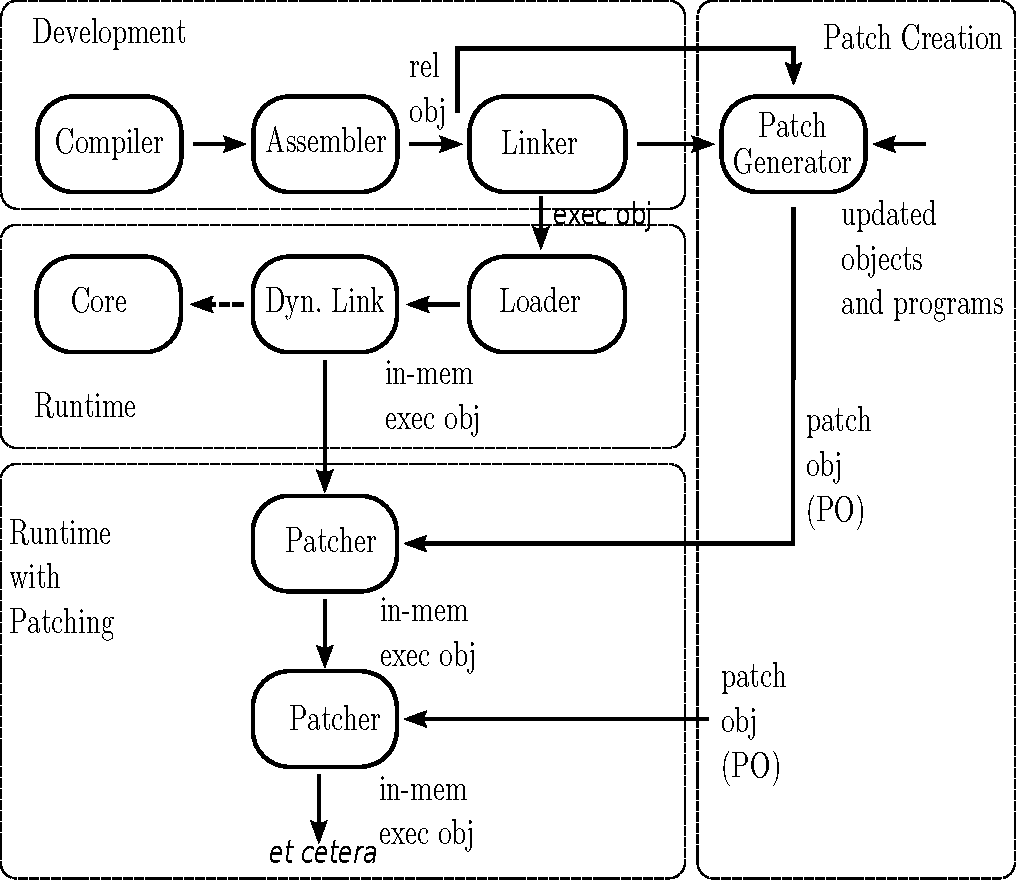
\includegraphics[width=3in]{./softwarelifecycle.pdf}
\end{figure}


  This document is intended to provide a users guide to Katana,
  insight into its inner workings, and discussion of its flaws and
  plans for the future. As the software is not complete, making use of
  Katana without understanding the inner workings and technical
  shortcomings is not recommended. Nevertheless, the only sections of
  this document necessary for ``Users' Guide'' purposes are 
  \hyperref[sec-3.2]{``What Katana Does''}, \hyperref[sec-3.3]{``What Katana Does Not Do (Yet)''}, and most importantly 
  \hyperref[sec-3.5]{``How to Use Katana For Hotpatching''}.
 
  This document is a work in progress. It is not a polished guide yet.

\section{General Usage Information}
\label{sec-2}

\subsection{Shell}
\label{sec-2.1}

   If Katana is not passed an argument indicating one of the
   hot-patching commands (described later in  \hyperref[sec-3.5]{*How to Use Katana For Hotpatching}), then it is assumed to be operating as a shell. If it
   is provided an argument, that argument is taken as the name of a
   file to read shell commands from. Otherwise commands are read from
   stdin using the readline library. 
\subsubsection{Syntax and Data Model}
\label{sec-2.1.1}

    The Katana shell syntax is very simple. There are no control flow
    structures, only commands and variables. A line is terminated by a
    semicolon (;) or a newline character. Each line may be either
    blank, contain exactly one COMMAND, or contain an ASSIGNMENT.

    A COMMAND is of the form COMMAND$_{\mathrm{IDENTIFIER}}$ PARAM PARAM PARAM \ldots{}., where
    tokens are seperated by spaces and the number of PARAMs depends on
    the command.

    An ASSIGNMENT is currently of the form VARIABLE=COMMAND although
    in the future it may be possible to write other sorts of
    assignments.

    A VARIABLE reference consists of a dollar-sign (\$) followed by a
    letter or underscore followed by any number of letters,
    underscores, or digits.

    A COMMAND$_{\mathrm{IDENTIFIER}}$ is one or more words which identify a
    COMMAND. In many cases a command is identified by only one word,
    but sometimes similar commands are grouped by sharing the first
    word in their identifier.

    A PARAM is a VARIABLE reference, STRING, or NUMBER

    A STRING is any literal beginning and ending with the character ``.

    A NUMBER is a decimal, hex, or float literal.

\begin{itemize}

\item Data Types\\
\label{sec-2.1.1.1}

     The following types of variables exist
\begin{itemize}
\item string
\item ELF
\item ELF section
\item raw data
\item array
\end{itemize}
\end{itemize} % ends low level
\subsubsection{Available Commands}
\label{sec-2.1.2}

\begin{itemize}

\item load\\
\label{sec-2.1.2.1}

     \emph{Usage}: \texttt{load FILENAME}\\
     \emph{Params}: FILENAME must a string literal or variable that can be interpreted
               as a string.\\
     \emph{Function}: Loads the data in the given file as an ELF object if
               possible. If not, loads it as raw data.

\item save\\
\label{sec-2.1.2.2}

     \emph{Usage}: \texttt{save VAR FILENAME}\\
     \emph{Params}: VAR must be a variable that can be interpreted as an ELF
               object or that can be interpreted as raw data. FILENAME must be a
               literal or variable that can be interpreted as a string.\\
     \emph{Function}: Saves VAR to FILENAME.

\item dwarfscript\\
\label{sec-2.1.2.3}

\begin{itemize}

\item dwarfscript emit\\
\label{sec-2.1.2.3.1}

      \emph{Usage}: \texttt{dwarfscript emit [SECTION] ELF OUTFILE}\\
      \emph{Params}: SECTION must be the name (string) of the section to write as
                Dwarfscript. If not specified it defaults to
                ``.eh$_{\mathrm{frame}}$''. ELF must be an ELF object. OUTFILE must
                be a string with the name of a file to write the resulting
                Dwarfscript to.\\
      \emph{Function}: Writes the Dwarfscript representation of the given
                  SECTION from the given ELF to OUTFILE.

\item dwarfscript compile\\
\label{sec-2.1.2.3.2}

      \emph{Usage}: \texttt{dwarfscript compile INFILE}\\
      \emph{Params}: INFILE must be a string containing the name of a file.\\
      \emph{Function}: Interprets the contents of the file named by INFILE
                  as Dwarfscript and compiles the Dwarfscript into
                  beinary form. Returns an array with 3 items
                  0: raw data for .eh$_{\mathrm{frame}}$ 
                  1: raw data for .eh$_{\mathrm{frame}}$$_{\mathrm{hdr}}$
                  2: raw data for .gcc$_{\mathrm{except}}$$_{\mathrm{table}}$.
\end{itemize} % ends low level

\item extract\\
\label{sec-2.1.2.4}

\begin{itemize}

\item extract section\\
\label{sec-2.1.2.4.1}

      \emph{Usage}: \texttt{extract section ELF SECTION\_NAME}
      \emph{Params}: ELF must be an ELF object. SECTION$_{\mathrm{NAME}}$ must be a
                string. 
      \emph{Function}: Returns the data and header information for the
                  specified section

\item extract section$_{\mathrm{data}}$\\
\label{sec-2.1.2.4.2}

      \emph{Usage}: \texttt{extract section ELF SECTION\_NAME}
      \emph{Params}: ELF must be an ELF object. SECTION$_{\mathrm{NAME}}$ must be a
                string. 
      \emph{Function}: Like extract section except extracts only the raw
                 data stored in the section and not any header information.
\end{itemize} % ends low level

\item replace\\
\label{sec-2.1.2.5}

\begin{itemize}

\item replace section\\
\label{sec-2.1.2.5.1}

      \emph{Usage}: \texttt{replace section ELF SECTION\_NAME NEW\_SECTION}
      \emph{Params}: ELF must be an ELF object. SECTION$_{\mathrm{NAME}}$ must be a
      string. NEW$_{\mathrm{SECTION}}$ must be either an ELF section or raw data.
      \emph{Function}: Replaces the section with the name SECTION$_{\mathrm{NAME}}$ in
      the oject ELF with the data from NEW$_{\mathrm{SECTION}}$. Section headers
      are replaced if NEW$_{\mathrm{SECTION}}$ is able to provide them, but not if
      it is only raw data.
                   

\item replace raw\\
\label{sec-2.1.2.5.2}

      \emph{Usage}: \texttt{replace raw ELF OFFSET NEW\_DATA}
      \emph{Params}: ELF must be an ELF object. ADDRESS must be an
                integer. NEW$_{\mathrm{DATA}}$ must be raw data.
      \emph{Function}: Replaces the raw data at OFFSET in the ELF object
                  with NEW$_{\mathrm{DATA}}$. OFFSET must refer to a location in an
                  existing section.
\end{itemize} % ends low level

\item info\\
\label{sec-2.1.2.6}

\begin{itemize}

\item info eh\\
\label{sec-2.1.2.6.1}

      \emph{Usage}: \texttt{info eh ELF [OUTFILE]}
      \emph{Params}: ELF must be an ELF object. OUTFILE, if present, must
                be the name of a writable file (which may or may not
                exist yet). 
      \emph{Function}: Prints out information about the exception-handling
                  structures in ELF. If OUTFILE is present, this
                  information is written to it.
\end{itemize} % ends low level

\item hash\\
\label{sec-2.1.2.7}

\begin{itemize}

\item hash elf\\
\label{sec-2.1.2.7.1}

      \emph{Usage}: \texttt{hash elf STR}
      \emph{Params}: STR must be a string.
      \emph{Function}: Prints the result of running elf$_{\mathrm{hash}}$ (from libelf)
                  on the string.
                  
\end{itemize} % ends low level

\item patch\\
\label{sec-2.1.2.8}

\begin{itemize}

\item gen\\
\label{sec-2.1.2.8.1}

      \emph{Usage}: \texttt{patch gen OLD\_OBJECTS\_DIR NEW\_OBJECTS\_DIR EXECUTABLE}
      \emph{Params}: All three params are strings. The first two are the
                old and new object file directories respectively. The
                last is the name of the executable that can be found
                in both directories.
      \emph{Function}: Generates (and returns) a patch object ELF.

\item apply\\
\label{sec-2.1.2.8.2}

      \emph{Usage}: \texttt{patch apply PO PID}
      \emph{Params}: The PO parameter should be an ELF patch object. PID
                should be the (integer) pid of the process that PO is
                to be applied to.
      \emph{Function}: Applies the patch object PO to the running process
                  described by PID.
\end{itemize} % ends low level

\item ! (shell command)\\
\label{sec-2.1.2.9}

     The rest of the line following by ! is executed in a shell.
\end{itemize} % ends low level
\subsubsection{History}
\label{sec-2.1.3}

    Command history is saved using libreadline in \texttt{\$HOME/.katana\_history}.
\section{Hotpatching}
\label{sec-3}

\subsection{Other Systems}
\label{sec-3.1}

   There are other hotpatching systems in existence. The curious are
   invited to explore Ginseng and Polus. Both of these systems parse
   the source code, which adds significant complexity to them and
   results in significant programmer annotation of the code to give
   hints to the systems. Ginseng uses complicated type-wrappers
   when patching variables which does not fit cleanly with existing
   executables and has some impact on the performance of the
   software. Ginseng is considerably more mature than Katana,
   however. Neither system is production ready, but Ginseng is probably
   closer than Katana at the moment.

   The system most like Katana in many ways is KSplice, and the curious
   reader is definitely invited to investigate. KSplice patches the
   kernel and not userland, does not attempt to patch variables, and
   creates patches as kernel modules rather than working towards a
   general ELF-based patch format.
\subsection{What Katana Does}
\label{sec-3.2}

\begin{itemize}
\item Runs on x86 and x86-64
\item Generates patches for simple programs
\item Applies simple patches
\end{itemize}
\subsection{What Katana Does Not Do (Yet)}
\label{sec-3.3}

\begin{itemize}
\item Patch any major programs: it has not yet been demonstrated on
     anything more than toy examples
\item Provide any method to handle opaque data it cannot patch (void*,
     situations where which action a user would prefer is unclear, etc)
\item Patch previously patched processes
\item Provide robust operation
\item Run on any architectures other than x86 and x86-64
\item Tested on any operating system besides GNU/Linux
\item Allow for calls in patched code to previously unused functions
\item Work for programs which actually make use of some of the large
     code model features of the x86-64 ABI.
\item And much more
\end{itemize}
   See \hyperref[sec-3.14]{Roadmap} for more things which are not complete

\subsection{What Katana May Never Do}
\label{sec-3.4}

\begin{itemize}
\item Work on any binary formats besides ELF
\end{itemize}
\subsection{How to Use Katana For Hotpatching}
\label{sec-3.5}

   Katana is intended to be used in two stages. The first stage
   generates a patch object from two different versions of an
   treee. By an object tree, we mean the set of object files (.o files)
   and the executable binary they comprise. Katana works completely at
   the object level, so the source code itself is not strictly
   required, although all objects must be compiled with debugging
   information. This step may be done by the software vendor. In the
   second stage, the patch is applied to a running process. The
   original source trees are not necessary during patch application, as
   the patch object contains all information necessary to patch the
   in-memory process at the object level. It is also possible to view
   the contents of a patch object in a human-readable way for the
   purposes of sanity-checking, determining what changes the patch
   makes, etc.
\subsubsection{Preparing a Package for Patching Support}
\label{sec-3.5.1}

     Katana aims to be much less invasive than other hot-patching system
     and require minimal work to be used with any project. It does,
     however, have some requirements.\\
\subsubsection{Source Code Practices}
\label{sec-3.5.2}

    Katana does not look at the source code, therefore unlike several
    other hotpatching systems, it does not require any annotation in
    the source code. There are, however, some best practices to
    follow.
\begin{itemize}
\item Avoid the use of \texttt{void*} at least for global variables (since
      Katana does not currently patch local variables, preferring to
      wait until any functions using changed variables are no longer
      on the stack). Since it is typeless and opaque, it is very hard
      to analyze and patch.
\item Avoid unnamed types. i.e., instead of \texttt{typedef struct \{...\} Foo;}
      use \texttt{typedef struct Foo\_ \{...\} Foo;}.
\item Avoid accessing structure members by offsets instead of by the
      member names. As long as you keep all the code where you do this
      up to date, it should not be a problem, but katana cannot detect
      when you do this.
\end{itemize}
\subsubsection{Compilation/Linking}
\label{sec-3.5.3}

    Required CFLAGS:
\begin{itemize}
\item -g
\end{itemize}
    Recommended CFLAGS:
\begin{itemize}
\item -ffunction-sections
\item -fdata-sections
\end{itemize}
    Recommended LDFLAGS:
\begin{itemize}
\item --emit-relocs
\end{itemize}
\subsubsection{To Generate a Patch}
\label{sec-3.5.4}

    Let the location of your project be /project. You must have two
    versions of your software available: the version identical to the
    running software which must be hotpatched, call it v0, and the
    version to which you wish to hotpatch the running software, call it
    v1. Let foo be the name of your program. Then /project/v0/foo must
    exist and /project/v0 must also contain (possibly in
    subdirectories) all of the object files which contributed to
    /project/v0/foo. The source code itself is immaterial, as Katana
    does not parse it. Similarly, /project/v1/foo must exist and
    /project/v1 contain all of the object files contributing to
    /project/v1/foo. Katana is then invoked as

    \texttt{katana [OPTIONS] -g [-o OUTPUT\_FILE] /project/v0 /project/v1 foo}

    or more formally

    \texttt{katana [OPTIONS] -g [-o OUTUT\_FILE] OLD\_OBJECTS\_DIR NEW\_OBJECTS\_DIR EXECUTABLE\_NAME}

    If \texttt{-o OUTPUT\_FILE} is not specified, the output file will be \texttt{OLD\_OBJECTS\_DIR/EXECUTABLE\_NAME.po}
\subsubsection{To Apply a Patch}
\label{sec-3.5.5}

    The process to be patched is running with a pid of PID. It can be
    patched from its current version to a more recent version by the
    Patch Object (PO) file PATCH. Katana is then invoked as

    \texttt{katana [OPTIONS] -p [-s] PATCH PID}

    If all goes well, the patcher will run, print out some status
    messages, and leave your program in better state than it found
    it. The optional -s flag tells Katana to stop the target program
    after patching it and detaching from it. This is mostly of use for
    debugging Katana.
\subsubsection{To View a Patch}
\label{sec-3.5.6}

    One of the goals of Katana and its Patch Object (PO) format is to
    increase the transparency of patches: a user about to apply a patch
    should know what it will do. This goal is not yet fully realized,
    but it is possible to view some information about a patch with

    \texttt{katana [OPTIONS] -l PATCH}
\subsubsection{Options}
\label{sec-3.5.7}

    The following options may be passed to katana regardless of whether
    one is generating, applying, or viewing a patch:
\begin{itemize}
\item -c CONFIG
      where CONFIG is the name of a configuration file to load
\end{itemize}
\subsubsection{Configuration Files}
\label{sec-3.5.8}

    Note that this feature is a work in progress. There isn't much you
   can do with configuration files right now and the information here
   may be out of date. Please do not rely on it.

    Katana loads configuration files as follows. Configuration files
    loaded later in the sequence may overwrite settings from files
    earlier in the sequence.
\begin{itemize}
\item \emph{etc/katana     + \~{}}.katana
\item \~{}/.config/katana
\item ./katana
\item any file specified with -c
\end{itemize}
    Configuration files are written in JSON. The JSON requirement that
    strings be quoted is relaxed (i.e. anything is assumed to be a
    string unless it can be interpreted otherwise). The following
    properties are recognized:
\begin{itemize}
\item maxWaitForPatching <INTEGER>
      This value specifies the maximum number of seconds to wait for
      the target to enter a safe state.
\item flags <OBJECT>
      The value of flags should be an object which may contain the
      following properties, all of which should be bool-valued:

\begin{itemize}
\item checkPtraceWrites
        Whenever something is written into the target memory, read the
        value back out and verify that it was written correctly. This
        has a performance penalty, but does provide some more robust
        error checking, although it should not be necessary.
\end{itemize}

\end{itemize}
\subsubsection{See Also}
\label{sec-3.5.9}

\begin{itemize}
\item The katana manpage (although the information in this document is
      considerably more extensive than in the manpage)
\item S. Bratus, J. Oakley, A. Ramaswamy, S. Smith,
      M. Locasto. \emph{Katana: Towards Patching as a Runtime part of the       Compiler-Linker-Loader Toolchain}. International Journal of
      Secure Software Engineering (IJSEE). 1, 3 (2010).
\end{itemize}
\subsection{Patch Object Format}
\label{sec-3.6}

   We have developed a patch object (PO) format which we hope will
   eventually pave the way for a standardized vendor-neutral patch
   format for hotpatching. We are not advancing our format as such,
   but it embodies some of the principles which we think are
   important. Why should patching not be a part of the ABI and of the
   standard toolchain?
\begin{itemize}
\item A PO is a valid ELF file.
\item A PO utilizes DWARF information to describe types, variables, and
     functions requiring patching.
\item A PO allows type transformations to be specified using a language
     based on the DWARF standard.
\end{itemize}
   Through the use of existing standards and well-structured ELF files
   utilizing a simple expression language for data patching, we aim to
   create patches that are easily examined (or modified) with existing
   tools. Relocatable objects containing new code and data which may
   be inserted at runtime are nothing new. This is the entire premise
   of the dynamic library. User-written functions which may have this
   code injection (in the case of patching data where the desired
   actions cannot be determined automatically) already exist as the
   .init and .fini sections. It is our view, however, that it is
   important to have a seperate patch format as opposed to patches
   merely being dynamic libraries which contain both the patch data
   and the logic to perform the patching (as is done by some other
   hotpatching systems). We view this as an unnecessary mixing of data
   and logic. The code to apply patches should live in one place on
   any given system, as most other executable content does.

   As an ELF object, our PO files contain the following non-standard
   sections.

\begin{itemize}
\item .text.new
     Contains new/modified functions
\item .rodata.new, .data.new
     new data
\item .unsafe$_{\mathrm{functions}}$
     Contains a simple listing (of symbol indices) of the functions in
     the binary to be patched which should not have activation records
     on the stack when patching is taking place.
\item .debug$_{\mathrm{info}}$
     Contains listings of the variables and functions which need to be
     patched using the DWARF data format. This section is standard and
     is used here with validly formatted data, but is used for
     patching instead of debugging. The use of the the .debug\_{} name is
     preserved for compatibility with libdwarf and tools such as
     readelf, objdump, dwarfdump capable of listing DWARF
     information. It can be, however, confusing and the name will
     likely change in the future.
\item .debug$_{\mathrm{frame}}$
     Like .debug$_{\mathrm{info}}$ a standard section used in a nonstandard way,
     see notes above about the naming. Contains an extended version of
     DWARF Call Frame Information which describes how various data
     structures are to be patched. The details are not properly
     documented at the moment, please email the Authors for more
     details if you would like further information.
\end{itemize}
\subsection{Patch Generation Process}
\label{sec-3.7}

   This section of the document is still under construction, but we
   hope that the information that is provided will be of some use.


   
\subsection{Configuration}
\label{sec-3.8}

   Note that this feature is a work in progress. There isn't much you
   can do with configuration files right now.
   
   Katana reads configuration files from (in order, with later
   configuration files overriding options found in earlier ones) from
   \texttt{/etc/katana}, \texttt{\textasciitilde{}/.katana}, \texttt{\textasciitilde{}/.config/katana}, and \texttt{./.katana}.

\subsection{Initializing the patch object}
\label{sec-3.9}

   Katana sets up a patch object ELF file with the necessary sections,
   see \hyperref[sec-3.6]{Patch Object Format}
\subsection{Comparing source trees}
\label{sec-3.10}

   High level view:
\begin{itemize}
\item Katana compare the old and new source trees, looking at the object (.o)
     files.
\item For object files which exist only in the new tree, their contents
     are added to the patch object being created.
\item For object files which exist only in the old tree, a warning
     about their removal is issued and nothing further is done.
\item For object files which exist in both trees, type diffing and
     function diffing are performed and the differences are written
     tot he patch object being created.
\end{itemize}
   A more detailed (although still very rough) algorithm:

\begin{verbatim}
Walk the old and new object trees in parallel
  For each pair of objects (corresponding old and new objects)
    If the new object does not exist
      Issue a warning and continue
    If the old object does not exist
      Add all functions and vars to patch
      Continue
    If the two objects are the same
      Continue
    If the two objects differ
      For every global variable in the old object
        Compare with matching variable in the new object
        If the two are a different type or the type struct changes
          Generate a type transformation for the patch
        If the variable initializers changed
          If the variable is const
            Add new data to the patch
          Else
            Generate a warning (can't determine automatically if
                the change should be applied)
        If anything related to the variable changed
          Find all functions using the variable
          Add them to the unsafe functions list
      For every global variable only in the new object
        Add it to the patch
      For every function in the old object
        Compare with matching function in the new object
          If the functions differ
            Add the new text to the patch
            Add the function to the unsafe functions list.
      For ever function only in the new object
        Add the function to the patch
Write out the patch ELF!
\end{verbatim}


\subsection{Type Diffing}
\label{sec-3.11}

   The general idea is that structures are examined for for added
   members, moved members, and changed members. If you need more
   detail than this, please contact the Authors.
\subsection{Function Diffing}
\label{sec-3.12}

   Functions are compared in an unsophisticated manner. The comparison
   is essentially byte-by-byte (i.e. no parsing of the machine
   instruction set is done). If bytes differ between the compiled
   version of the old function and the new function, then the function
   is assumed to need patching.  The one exception to this is that
   relocations are accounted for. If bytes differ at an address that
   is fixed up by relocations, the relocations are examined to make
   sure that they are for the same symbol. If in fact they are, then
   the function is deemed not to have changed. If the symbol referred
   to corresponds to a variable that has changed then it may need to
   be moved to be patched. In that event the function may in fact have
   to be modified, but it will be modified only to apply the
   relocations rather than as a patch to the function per se and thus
   the function diffing stage does not concern itself with whether
   referenced symbols have changed.
\subsection{Patch Application Process}
\label{sec-3.13}

   This section of the document is not yet written. It will provide a
   description of the internal process that Katana uses to apply a
   patch. Understanding it is not necessary for using Katana.

   The basic process is as follows

\begin{verbatim}
Read the patch file
Calculate versioning. This is currently not implemented.
Find malloc in the target, as we may need it
Calculate a safe state for the target (based on the unsafe functions list)
Wait for the target to reach a safe state
Map in necessary sections from the patch
Copy PLT and GOT to new locations as we may need to expand them
For each variable listed in the patch
  Apply the variable patch
For each function listed in the patch
 Apply the function patch
Apply necessary relocations
\end{verbatim}


\subsection{Roadmap}
\label{sec-3.14}

   This section is highly incomplete. Future goals include
\begin{itemize}
\item Better interaction with the heap and dynamically allocated variables
\item Better interaction with void*
\item More efficient use of .rodata
\item Patching already patched processes
\item Patch composition
\item Patch safety checking: make sure a patch actually corresponds to
     the process it's being applied to
\item Storing warnings from generation inside a patch
\end{itemize}
\section{DWARF Manipulation}
\label{sec-4}

  For information on how katana can be used specifically for DWARF
  manipulation, please see Dartmouth College Tech Report TR2011-680.
\section{Credits and Licensing}
\label{sec-5}

  Katana is under development at Dartmouth College and Copyright 2010
  Dartmouth College. It may be distributed under the terms of the GNU
  General Public License with attribution to Dartmouth College as
  specified in the file COPYING distributed with Katana. This document
  is Copyright 2010-2011 Dartmouth College and may be distributed
  under the terms of the GNU Free Documentation License as found in
  the file FDL which should have been distributed with this
  documentation. If it was not, it may be found at
  \href{http://www.gnu.org/licenses/fdl.txt}{http://www.gnu.org/licenses/fdl.txt}.

  Katana is being written by James Oakley and was designed by Sergey
  Bratus, James Oakley, Ashwin Ramaswamy, Michael Locasto, and Sean
  Smith.

\end{document}